\section{Optimización basada en gradientes con restricciones}

\subsection{Optimización con y sin gradientes}

La optimización paramétrica sin el uso de gradientes no es escalable para
problemas con un gran número de variables de diseño, como ocurre en problemas
de control óptimo, optimización topológica, o aprendizaje automático.

Los algoritmos libres de gradiente buscan el óptimo poblando el espacio de
diseño y evaluando la función objetivo en estos puntos. Sin embargo, al
introducir más variables de diseño, el espacio crece exponencialmente, así como
el número de puntos a evaluar.

\begin{figure}[h] \centering
	\centering
	\includesvg[width=0.6\textwidth]{./capitulos/metodologia/images/volume_curse_of_dimensionality_print}
	\caption{Crecimiento exponencial del número de puntos a poblar con el número de dimensiones.}
	\label{fig:hypercube}
\end{figure}

Asumiendo que la evaluación de cada punto tiene un coste computacional no
despreciable, el uso de estos algoritmos se vuelve inviable para problemas con
más de unas pocas decenas de variables de diseño. El volumen de un hipercubo
n-dimensional crece como:

\begin{equation}
	V = l^n
\end{equation}

donde $l$ es la longitud del lado y $n$ es la dimensión.


Los algoritmos basados en gradientes, en lugar de poblar el espacio de
diseño, lo navegan avanzando hacia el óptimo por un camino determinado por
el gradiente de la función objetivo respecto a las variables de diseño.

Mientras que el espacio de diseño crece exponencialmente en volumen con el
incremento de las variables de diseño, la distancia entre dos puntos dentro
de este volumen no lo hace de manera tan drástica. Para un hipercubo
n-dimensional, su diagonal viene dada por:

\begin{equation}
	d = l\sqrt{n}
\end{equation}

Nótese que el aumento no es exponencial con el número de dimensiones, ni
tan siquiera es lineal.

Si el número de iteraciones realizadas por el algoritmo de optimización
es proporcional a la longitud del camino entre los puntos inicial y final(óptimo),
entonces el coste computacional crece con la raiz del número de dimensiones, o
variables de diseño.

Esta estrategia permite la optimización de problemas con un gran número de
incógnitas. Por ejemplo, el modelo de lenguaje Llama-3.1-405b de Meta
utiliza 405 mil millones de variables \cite{dubey2024llama}, o parámetros como
se conocen en el contexto del aprendizaje automático.


\begin{figure}[h]
    \centering
    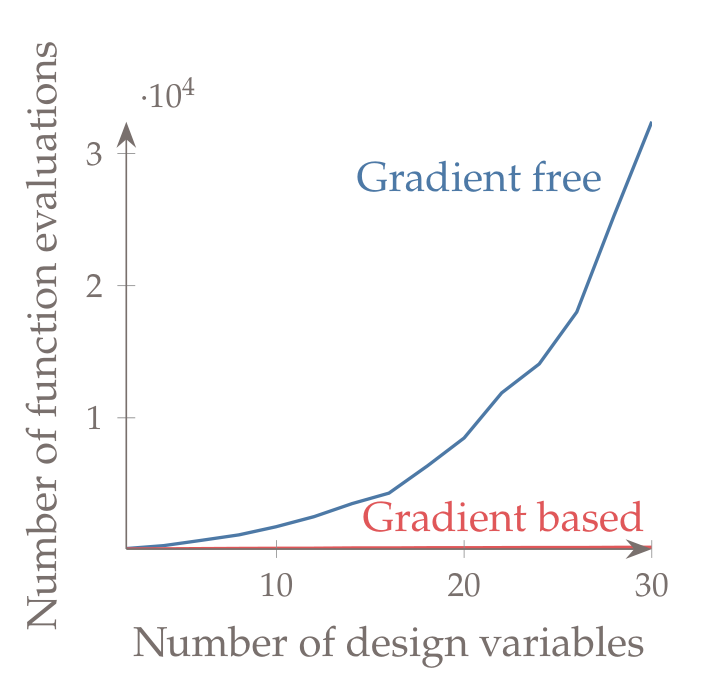
\includegraphics[width=0.4\textwidth]{./capitulos/metodologia/images/gradient_based_vs_gradient_free.png}
    \caption{Los algoritmos de optimización que emplean gradientes escalan mucho mejor con el número de variables de diseño. (Adaptado de Martins y Ning \cite{mdobook}, p. 22)}
    \label{fig:gradient_based_vs_gradient_free}
\end{figure}


\subsection{Restricciones}

La gran mayoría de los problemas en ingeniería requieren el uso de
restricciones en su formulación. Estas restricciones pueden ser de igualdad o
desigualdad y representan limitaciones físicas, económicas o de diseño que
deben satisfacerse durante el proceso de optimización.
